\section{Final Bootware Architecture}
\label{finalarch}

\autoref{image:finalarch} shows the final architecture of the bootware component.
At the bottom we can see six exemplary event plugins.
These are loaded at the beginning of the bootware execution by the plugin manager, shown on the left of \autoref{image:finalarch}.
For demonstrations purposes, \autoref{image:finalarch} shows a wider range of possible event plugins.
All these plugins provide some sort of input andd/or output mechanism for the bootware component.
The web service plugins could provide a web service interface.
This would allow other components to start the deploy and undeploy operations with web service calls.
Another possibility for interaction would be a \nom{command-line interface}{CLI} plugin that would make these operations accessible via a command-line interface.
A event logger plugin could be used to write all bootware events to a log file.
We can also imagine a event queue plugin that pushes all bootware events into some message queue so that they can be consumed by other components.
Finally, an undeploy trigger plugin could trigger the undeployment of the bootware and all running payloads when it receives a message from the ODE event queue.

All event plugins work by implementing event handlers for certain events published at the event bus, or by publishing events to the event bus themselves.
As we can see in the center of \autoref{image:finalarch}, the event bus and the state machine form the core of the bootware.
The event bus is responsible for distributing events between the various plugins and the state machine.
The state machine implements the entire bootstrapping process, as described earlier in \autoref{flow}.
At certain points during the bootstrapping process, operations are delegated to the plugin manager to load plugins, and to the infrastructure, connection, and payload plugins, shown at the top of \autoref{image:finalarch}.

The infrastructure, connection, and payload plugins implement the actual bootstrapping operations.
At the top, \autoref{image:finalarch} shows an exemplary result of these bootstrapping operations.
In this particular case, the infrastructure plugin started a VM, to which the connection plugin set up a communication channel.
The payload plugin then used this communication channel to provision the payload inside the VM.
During the bootstrapping procedure, events are sent from those plugins back to the event bus to be delivered to the loaded event plugins.


\begin{figure}[!htbp]
	\centering
	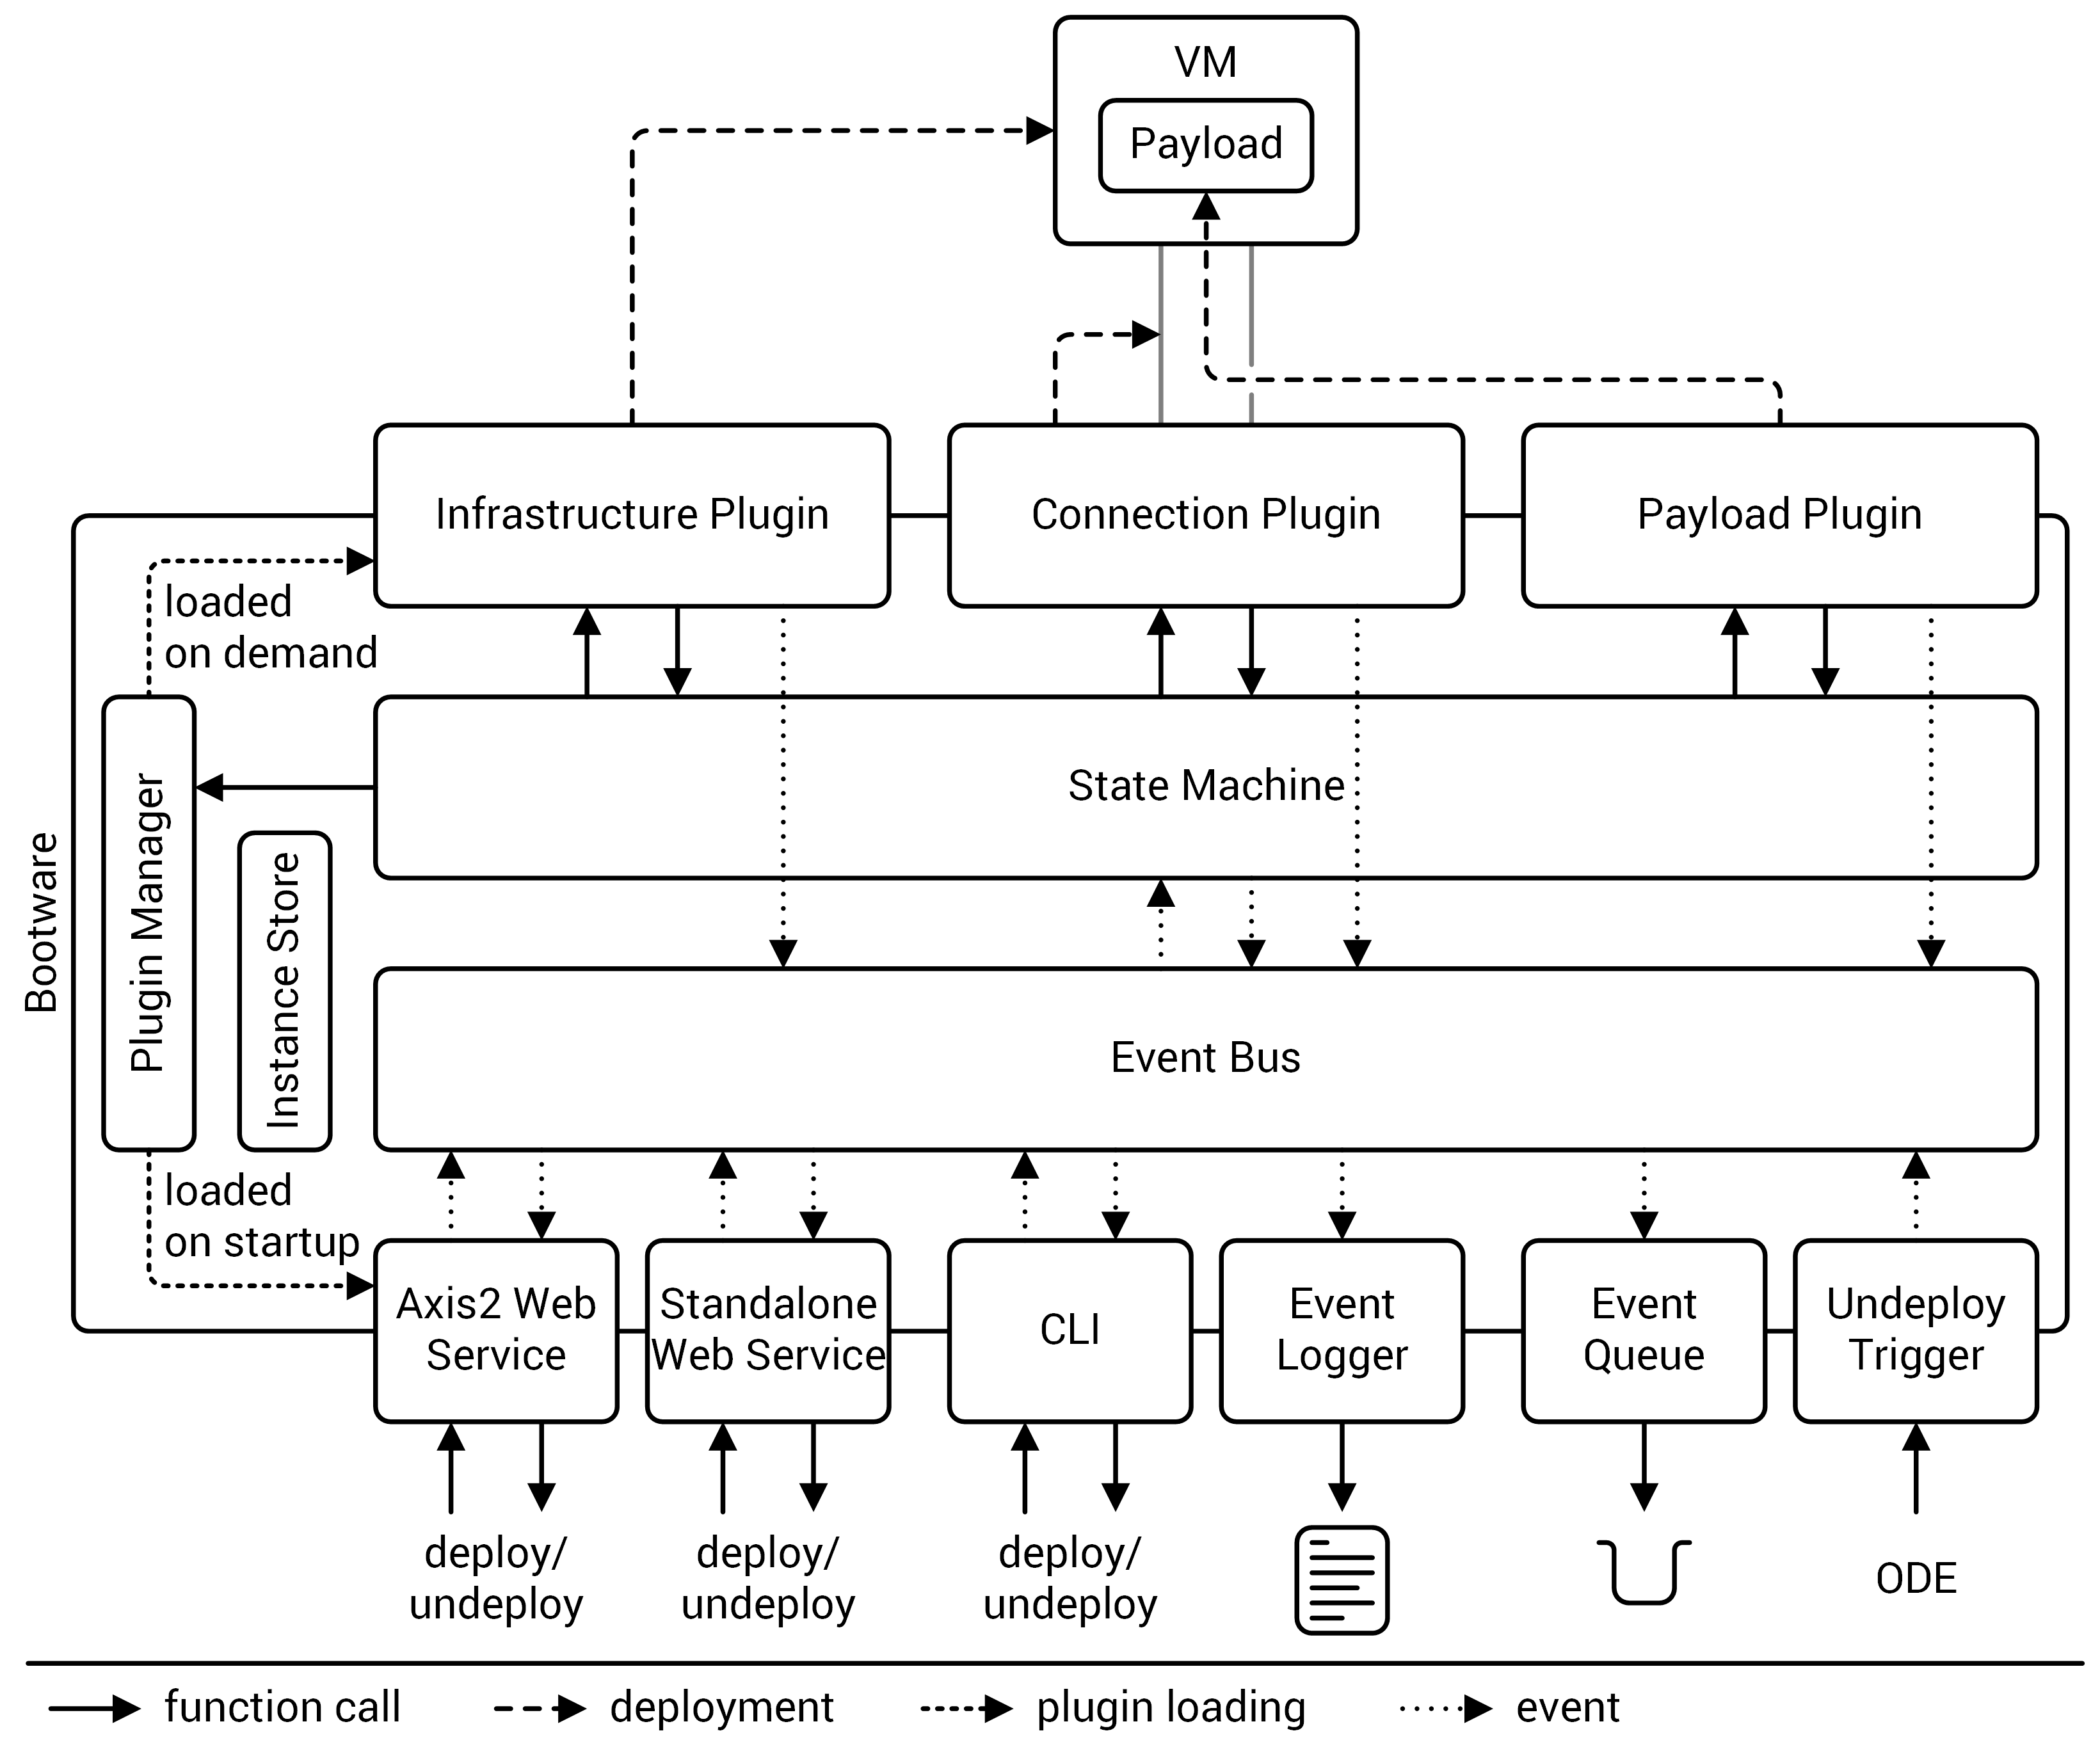
\includegraphics[resolution=600]{design/assets/final_bootware_architecture}
	\caption{The final architecture of the bootware component.}
	\label{image:finalarch}
\end{figure}
